\section{A Seiva da Árvore \ldots}\label{sec:seiva} %==========================

\begin{margintable}\vspace{.8in}\footnotesize
  \begin{tabularx}{\marginparwidth}{|X}
    Seção~\ref{sec:seiva}. A seiva da árvore\\
    Seção~\ref{sec:seiva}. A seiva da árvore\\
    Seção~\ref{sec:seiva}. A seiva da árvore\\
  \end{tabularx}
\end{margintable}

Lembro-me da primeira vez que vi o nome \LaTeX\ \ldots

Foi em uma chamada de um minicurso de alguma "semana de matemática" da 
universidade que fiz graduação.
O título era algo assim: "Introdução ao \LaTeX".

Eu estava a um semestre de concluir a graduação e pensei: 
\textit{
  "Rapaz \ldots acho que eles erraram esse minicurso. 
  Pra quê estudar látex em Matemática? 
  Isso está mais para Geografia."
}

\begin{marginfigure}
  \centering
  \href
  {
    https://www.globo.com/GloboRural/0,6993,EEC1703411-1935,00.html
  }
  {
    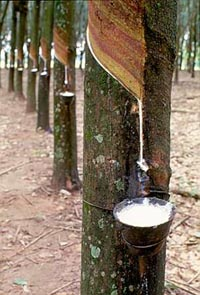
\includegraphics[width = 0.75\linewidth]{seringueira.jpg}
  }
  \caption{Isso é látex, não \LaTeX}
\end{marginfigure}

Sim! 
Eu pensei que estavam falando daquela substância espessa e branca que sai de 
algumas plantas (seringueira, por exemplo)!

Então, vamos deixar as coisas claras: não estamos falando de látex, mas de \LaTeX.

\begin{aviso}
  Aliás, como se pronuncia a palavra \LaTeX?
  Existem, pelo menos, duas maneiras de se pronunciar corretamente essa palavra:
  "\textit{LeiTéc}" ou "\textit{LaTéc}",ou seja, o som de \TeX{} ("Téc") é o 
  mesmo que em "\textbf{tec}nologia". 
  Particularmente, adoto a segunda opção.
  Evite, por amor a Deus, falar "\textit{Látecks}".
\end{aviso}

Falando nisso, a palavra \TeX, foi idealizada como sendo a junção de três letras
gregas: $\tau\epsilon\chi$.\footnote{%
  $\tau$ (tau), $\epsilon$ (épsilon) e $\chi$ (chi)
}
Esse núcleo grego gera palavras como \textit{arte} ($\small\tau\epsilon\chi\nu\eta$) 
ou mesmo \textit{tecnologia} ($\small\tau\epsilon\chi\nu o \lambda o \gamma\iota\alpha$).
Daí vem o espírito da palavra \TeX: unir uma arte (a tipografia) com a 
tecnologia (programação) para produzir documentos com uma beleza realmente ímpar.


